%!TEX root = ../thesis.tex
%*******************************************************************************
%*********************************** First Chapter *****************************
%*******************************************************************************

\chapter{Introduction}  %Title of the First Chapter

\ifpdf
     \graphicspath{{/Users/luyolomagangane/Documents/Academics/Figures/Chapter1/}}
\else
    \graphicspath{{Chapter1/Figs/Vector/}{Chapter1/Figs/}}
\fi


%********************************** %First Section  **************************************

\section{Overview} %Section - 1.1 

\emph{"... as they say, your model is only as good as the data you have. \newline So it all starts with the data ..."} \newline
\indent \indent - Nyalleng Moorosi, \emph{Deep Learning Indaba} (2017). \newline 

Artificial intelligence (AI) is the imitation of human-level intelligence by machines. Human beings are capable of extracting information from a passage of text and transforming that information into a mental model of objects and relationships between those objects. As stated by Nyalleng Moorosi, the model is only as good as the data you give it, this is true for both human mental models as well as machine constructed models. \newline 
Human models are often confined to a finite domain ~\citep{staab2010handbook}, for example a mental model might be one of the entertainment industry. The entertainment industry contains objects such as films, actors and actresses, characters and awards. These objects have relationships between them, such as "stared in", "worked along side", "a character in", and "was nominated for". Humans can use this model to easily reason about new relationships between the objects that weren't mentioned in passage of text. For example the text may say that Chadwick Boseman stared in a movie called Black Panther, and using that information we can reason that Chadwick Boseman "is an" actor. \newline
We use these models to read and understand other passages of text, in conversations with other people, and to help us answer questions. The set of objects and the relationships between them, within a domain, can be thought of as knowledge. Figure 1.1. shows what knowledge about the entertainment industry might look like. \newline

\begin{figure}
  	\caption{Objects and the Relationships between Them}
   	\centering
    	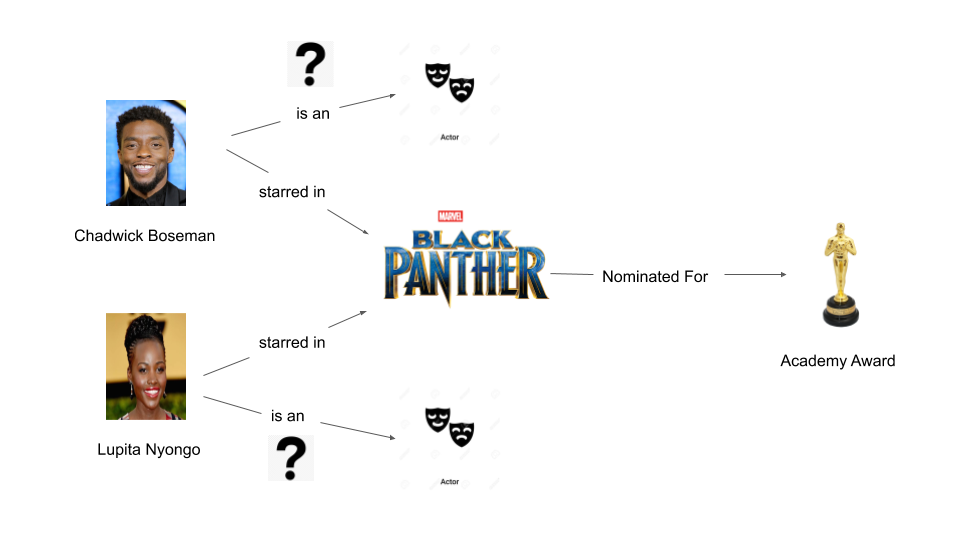
\includegraphics[width=\textwidth]{Objects_and_the_Relationships_Between_Them}
\end{figure}


\textbf{Challenges}. Reasoning about knowledge expressed in natural language ~\citep{minervini2019differentiable} is simple for humans, but trying to imitate this behaviour in computers reveals its underlying complexity. \newline 
The first task is providing a mechanism for perceiving syntax. Humans recognise text as sequences of words, and words as a sequence of characters. Characters can belong to different writing systems which can be dense - have a few characters used in a large number of combinations, or sparse - have a very large number of characters used in less combinations ~\citep{Hua2010}. A computer has to first be able to perceive these characters. \newline
The second task is even more challenging: semantics. Semantics is the meaning of words in language ~\citep{chomsky1955logical}. Semantics is what allows humans to understand each other in conversation, through written text, and through visual imagery. Semantics allow us to understand that an actor is a thing, and that things can have relationships with other things. Giving computers the capability to semantic understanding is very challenging because of the "messiness" of language. If a person is shown a word in the singular, and a word in the plural, for example "film" and "films" a person will most likely understand that there is not much difference in meaning between the two words, a computer may interpret them as having completely different meanings. Different words can also have similar meanings, for example "movie" and "film". Capturing this statistical similarity once again challenging for machines. And finally the order in which words are seen provides context, for example, the word "star" has completely different meaning in "Chadwick Boseman is a movie star" and "Black Panther looked up into the night sky an saw a star". \newline
The third task is organising information in such a way as to be able to reason about the knowledge it conveys. Humans typically use the few objects and relationships within a domain to infer new plausible relationships between objects. For computers, this sort information is organised in a database. 


% Link prediction with Latent Feature Models is the focus of this dissertation.



\nomenclature[z-cif]{$CIF$}{Cauchy's Integral Formula}                                % first letter Z is for Acronyms 
\nomenclature[a-F]{$F$}{complex function}                                                   % first letter A is for Roman symbols
\nomenclature[g-p]{$\pi$}{ $\simeq 3.14\ldots$}                                             % first letter G is for Greek Symbols
\nomenclature[g-i]{$\iota$}{unit imaginary number $\sqrt{-1}$}                      % first letter G is for Greek Symbols
\nomenclature[g-g]{$\gamma$}{a simply closed curve on a complex plane}  % first letter G is for Greek Symbols
\nomenclature[x-i]{$\oint_\gamma$}{integration around a curve $\gamma$} % first letter X is for Other Symbols
\nomenclature[r-j]{$j$}{superscript index}                                                       % first letter R is for superscripts
\nomenclature[s-0]{$0$}{subscript index}                                                        % first letter S is for subscripts

%********************************** %Second Section  *************************************
\section{Modelling Techniques} %Section - 1.2

\subsection{Latent Feature Modelling} % Latent Feature Modelling
Entities and relations are words that can be represented as real-valued vectors [references]. These real-valued vectors form part of a euclidean embedding space that represents a knowledge domain [references]. The entity and relational vectors can be randomly generated, or be pre-computed to capture semantic meaning [references]. A classification model can then be constructed that generates a probability distribution over probable facts within the knowledge domain. In order to compute the probability distribution, a number of latent feature modelling techniques are used, including tensor factorisation [references], circular correlations [reference] and convolutional feature maps [reference]. These methods can broadly be defined as linear and nonlinear. Attractive attributes of linear latent models are their simplicity, ease of implementation and computational efficiency. Linear latent models however suffer from a lack of expressiveness and struggle to model complex, contradictory or incoherent relationships between entities. Nonlinear latent feature models are able to produce more expressive latent feature sets, and so more adept at capturing complex relationships. Nonlinear models however suffer from computational inefficiency and poorly generalise concepts. \newline
\subsection{Graph Feature Modelling} % Graphical Modelling
In Graph Feature Modelling, Knowledge Graphs (KG) are used to model domains. KGs are composed of nodes and edges, where nodes represent entities and edges represent relations. The graphical structure then captures local, quasi-local and global domain properties. This global structure exhibits particular properties about relations within the domain, characteristics of the entities of the domain, and local entity-relational sub-structures. These graph structure properties are used in supervised [reference] and unsupervised [Graph Infomax] settings for SRL tasks such as link prediction and entity-resolution. The directional nature of edges in graph structures (uni-relational and bi-relational) is also exploited to further enhance the fulfillment of SRL tasks [reference]. The assumption in general in KGs is that similar entities will be collocated within a local and quasi-local regions, and that global similiarty patterns between entities will be captured by the ensemble of all paths between entities. Link-based clustering [reference] is thus used at all these structural scopes, and supports link prediction and entity-resolution tasks. 
\subsection{Inductive Probabilistic Logic Programming}  % Inductive Probabilistic Logic Programming
Inductive logic programming uses ontological facts to discover new facts within a knowledge domain [reference]. logical rules check for things such as consistency. coherence and contradiction. Knowledge domains are implemented as knowledge bases (KB) that follow the resource description framework [reference]. KBs initialised in two steps: fact recording and materialisation - the discovery of new facts by running logical queries over the entire KB. KBs are extremely computationally demanding [reference], they also suffer from an inflexibility in modelling complex relationships due to their exactness, a fact is either true or false with no measure of ambiguity. Probabilistic logic programming languages have recently gained a lot of attention as flexible alternatives to logic programming languages as they are able to capture uncertainty in logical assertions through by modelling probability distributions over KB facts using stochastic variational inference. These models are thus more flexible in modelling complex relationships, and are also more computationally efficient [reference]. Inductive probabilistic logic programming has recently gained a lot of research attention due to it's capability of extending probabilistic logic programming languages with the capability of knowledge discovery. 

%********************************** % Third Section  *************************************
\section{Link Prediction with Latent Feature Models}  %Section - 1.3 
\label{section1.3}
\subsection{Knowledge Graph Latent Feature Models}
Link prediction with latent feature models involves building entity-relational representations from the nodes and edges of knowledge graphs expressed as subject-predicate object triples. These triples explicitly model facts within a knowledge domain. Entity and relational representations are commonly implemented as real-valued vectors. The vectors are then combined using compositional models, such as neural networks, to produce latent relational representations that can be used to compute the likelihood of plausible relationships between entities. The domain can be said to represent a multidimensiona embedding space into which the entities and relations are projected. Knowledge graph based latent feature modelling approaches are similar to semantic embedding representations [rerferenc]. They differ in that knowledge graph approaches explicitly model entity-relational interactions,  and semantic embedding approaches rely on the distributional word representation techniques [reference], relying on Skip-Gram [reference] and Contious Bag of Words [reference] to generate word representations. This is an implicit modelling of relationships between word vectors. \newline
\subsection{Factorisation of Latent Feature Models}
Factorisation attempts to model concepts between words, these facts are discovered using unsupervised techniques such as singular value decomposition. In the case of knowledge graphs, we obtain explicit representations of these concepts and can use them for entity-relational transformations that represent intermediate relational concepts that can then be used to determine plausible relationships when tested against subject entities.
Tensor factorisation is an approach used for link prediction with latent feature models. It involves modelling entity relationships as matrix slices that comprise a relational tensor. The entity between entities is then computed using a bilinlear tensor product [reference], where the inner product of the object entity is taken with the matrix relational representation before an inner product of the resultant representation is taken with the subject entity. Bilinear tensor factorisation models are efficient in their number of parameters but lack expressiveness. Multilayer perceptrons have been used to overcome the lack of expressiveness however often suffer from overfitting. Recently convolutional neural networks have been proposed to allow expressive factorisation [references], do not suffer from overfitting and remain computationally efficient. \newline
\subsection{Other of Latent Feature Modelling Approaches}
A number of alternative approaches to latent feature model factorisation have been proposed for link prediction, including circular correlation [reference], holographic entity-relational transformations [reference], toroidal representations [reference]. The rest of this dissertation focuses on factorisation of latent feature models, with the explicit representation of relational concepts. \newline

\nomenclature[z-DEM]{DEM}{Discrete Element Method}
\nomenclature[z-FEM]{FEM}{Finite Element Method}
\nomenclature[z-PFEM]{PFEM}{Particle Finite Element Method}
\nomenclature[z-FVM]{FVM}{Finite Volume Method}
\nomenclature[z-BEM]{BEM}{Boundary Element Method}
\nomenclature[z-MPM]{MPM}{Material Point Method}
\nomenclature[z-LBM]{LBM}{Lattice Boltzmann Method}
\nomenclature[z-MRT]{MRT}{Multi-Relaxation 
Time}
\nomenclature[z-RVE]{RVE}{Representative Elemental Volume}
\nomenclature[z-GPU]{GPU}{Graphics Processing Unit}
\nomenclature[z-SH]{SH}{Savage Hutter}
\nomenclature[z-CFD]{CFD}{Computational Fluid Dynamics}
\nomenclature[z-LES]{LES}{Large Eddy Simulation}
\nomenclature[z-FLOP]{FLOP}{Floating Point Operations}
\nomenclature[z-ALU]{ALU}{Arithmetic Logic Unit}
\nomenclature[z-FPU]{FPU}{Floating Point Unit}
\nomenclature[z-SM]{SM}{Streaming Multiprocessors}
\nomenclature[z-PCI]{PCI}{Peripheral Component Interconnect}
\nomenclature[z-CK]{CK}{Carman - Kozeny}
\nomenclature[z-CD]{CD}{Contact Dynamics}
\nomenclature[z-DNS]{DNS}{Direct Numerical Simulation}
\nomenclature[z-EFG]{EFG}{Element-Free Galerkin}
\nomenclature[z-PIC]{PIC}{Particle-in-cell}
\nomenclature[z-USF]{USF}{Update Stress First}
\nomenclature[z-USL]{USL}{Update Stress Last}
\nomenclature[s-crit]{crit}{Critical state}
\nomenclature[z-DKT]{DKT}{Draft Kiss Tumble}
\nomenclature[z-PPC]{PPC}{Particles per cell}